\documentclass[11 pt]{article}
%% PAQUETES DISPONIBLES
\usepackage[utf8]{inputenc} %codificación 
\usepackage[spanish, es-lcroman]{babel} %idioma
\usepackage{float}% para usar H
\usepackage{amsmath} %matemáticas
\usepackage{empheq} 
\usepackage{amsthm}
\usepackage{nccmath}
\usepackage{mathrsfs} %% curly letters 
\usepackage{mathtools} %matemáticas
\usepackage{physics} %diferenciales
\usepackage{blindtext}%texto de relleno
\usepackage{amsfonts} %matemáticas
\usepackage{amssymb} %matemáticas
\usepackage{makeidx} 
\usepackage{graphicx} %imágenes
\usepackage[a4paper, margin=2cm, scale=0.8]{geometry}
\usepackage{wrapfig} %figuras alrededor de texto
\usepackage{caption} %subtítulos de figuras
\usepackage{setspace}%interlineado 
\usepackage{array}% entorno array
\usepackage{ragged2e} %alineación 
\usepackage{tabularx} %entorno tabularx (tablas con ancho fijo)
\usepackage{fancyhdr} %cabeceros y pies de página
\usepackage{multirow} %combinar columnas y filas en una tabla
\usepackage{longtable} %mediante este paquete podemos separar una tabla larga en varias que ocupen las páginas necesarias.
\usepackage[table]{xcolor} %con este paquete cambiamos el color de los objetos y concretamente de la opción de las tablas.
\usepackage{enumitem}%enumeraciones personalizadas
\usepackage{subcaption}%subtítulos de figuras y subfiguras
\usepackage{hyperref} % este paquete siempre debemos colocarlo al final 
\usepackage{multicol} %columnas
\usepackage{parskip} %espaciado entre párrafos
\usepackage[rightcaption]{sidecap} %subtítulos alrededor de figuras
\usepackage{ifthen} %condicionales
\usepackage{xparse} % Para manejar parámetros opcionales

% FORMATO PARA FIGURAS Y SUBFIGURAS
\DeclareCaptionFormat{format1}{
%#1=label, #2 = separator, #3 = text
	\textbf{#1#2}#3
}

\DeclareCaptionFormat{format2}{
%#1=label, #2 = separator, #3 = text
\textsc{#1#2}#3
}  

\DeclareCaptionLabelSeparator{parentesis}{$)\,$ }
\DeclareCaptionStyle{subfigura}{
format = format1, 
justification = raggedright, 
labelsep = parentesis,
font = {color = black, huge},
}
\DeclareCaptionStyle{subfigura2}{
format = format1, 
justification = raggedright, 
labelsep = parentesis,
font = {color = black, Large},
}
%% COMANDO PARA TITULOS
\NewDocumentCommand{\settitle}{O{0} O{0} m}{
	% [nombre del autor][nombre de la asignatura]{titulo}
\ifthenelse{\equal{#1}{0}}{}{\author{#1}}
\ifthenelse{\equal{#2}{0}}
	{
	\date{\vspace*{1em}
	\hrule
	\vspace*{1em}}}
	{\date{\Large{UAM - #2}\vspace*{1em}
	\hrule
	\vspace*{1em}}
	}
\title{\Huge \textbf{#3}}
}

%% COMANDO PARA ELEGIR FORMATO
\NewDocumentCommand{\setformat}{O{0.8\textwidth} O{centering} m}
% [ancho de figuras][alineacion de figuras]{cabecero derecho}
% tras elegir este comando no olvidar usar \brightmode y \darkmode para cambiar aplicar el formato deseado
{
%FORMATO PARA PÁGINAS OSCURAS Y CLARAS
\fancypagestyle{claroi}{
\fancyhf[]{}
\fancyhead[L]{\color{black}\textsc{UAM}}
\fancyhead[R] {\color {black}\textsc{#3}}
\fancyfoot[C]{\color{black}\thepage}
\setlength{\headheight}{18pt} 
\renewcommand{\headrulewidth}{0.75pt}
\renewcommand{\headruleskip}{-0.5em}
\renewcommand{\headrule}{\hbox to\headwidth{%
    \color{black}\leaders\hrule height \headrulewidth\hfill}}
  \renewcommand{\footrulewidth}{0pt}
}

\fancypagestyle{oscuroi}{
\fancyhf[]{}
\fancyhead[L]{\color{white}\textsc{UAM}}
\fancyhead[R] {\color {white}\textsc{#3}}
\fancyfoot[C]{\color{white}\thepage}
\renewcommand{\headrulewidth}{0.75pt}
\renewcommand{\headruleskip}{-0.5em}
\renewcommand{\headrule}{\hbox to\headwidth{%
    \color{white}\leaders\hrule height \headrulewidth\hfill}}
  \renewcommand{\footrulewidth}{0pt}
}
\DeclareCaptionStyle{figura_claro_custom}{
format = format1, 
justification = #2,
font = {color = black,small},
name = Fig.,
width = #1
}

\DeclareCaptionStyle{figura_oscuro_custom}{
format = format1, 
justification = #2,
font = {color = white,small},
name = Fig.,
width = #1
}

\DeclareCaptionStyle{tabla_claro_custom}{
format = format1, 
justification = #2,
font = {color = black,small},
name = Tabla,
width = #1
}

\DeclareCaptionStyle{tabla_oscuro_custom}{
format = format1, 
justification = #2,
font = {color = white,small},
name = Tabla,
width = #1
}


% MODO OSCURO O CLARO
\def\darkmode{
\pagecolor{black}
\color{white}
\pagestyle{oscuroi}
\captionsetup[figure]{style=figura_oscuro_custom}
\captionsetup[table]{style = tabla_oscuro_custom}
\hypersetup{
colorlinks = true,%% atento a la separación con comas
%% si colocas colorlinks = false aparecen cajas alrededor de los links pero no se ven ni con texmaker ni los navegadores convencionales,en cambio sí que se ve con adobe acrobat reader. 
linkcolor = cyan, 
citecolor= cyan,
filecolor = magenta, 
urlcolor = cyan,
pdfpagemode = FullScreen,
urlbordercolor = {1 0 0},
linktocpage = false, %% si es verdadero son las páginas del índice las que quedan referenciadas
}
}
\def\brightmode{
\pagecolor{white}
\color{black}
\pagestyle{claroi}
\captionsetup[figure]{style=figura_claro_custom}
\captionsetup[table]{style = tabla_claro_custom}
}
\hypersetup{
colorlinks = true,%% atento a la separación con comas
%% si colocas colorlinks = false aparecen cajas alrededor de los links pero no se ven ni con texmaker ni los navegadores convencionales,en cambio sí que se ve con adobe acrobat reader. 
linkcolor = blue, 
citecolor= blue,
filecolor = magenta, 
urlcolor = blue,
pdfpagemode = FullScreen,
urlbordercolor = {1 0 0},
linktocpage = false, %% si es verdadero son las páginas del índice las que quedan referenciadas
}
}
\urlstyle{same}
\definecolor{coolgreen}{RGB}{15, 219, 97}
%QUITAR NÚMERO EN UNA PÁGINA
\def\resetnumpagetitle{
\thispagestyle{empty}
\newpage
\setcounter{page}{1}
}
%% COMANDOS MATEMÁTICOS
\DeclareMathOperator{\rot}{\textrm{\textbf{rot}}}
\DeclareMathOperator{\diver}{\textrm{\textbf{div}}}
\renewcommand{\grad}{\textrm{\textbf{grad}}} 
\newcommand{\appeq}{\backsimeq} %%aproximaciones
\newcommand{\FT}[1]{\mathcal{F}\{#1\}} % Transformada de Fourier 
\newcommand{\LT}[1]{\mathcal{L}\left\{ #1 \right\}} %Transformada de Laplace
\newcommand{\BLT}[1]{\mathcal{B}\left\{#1\right\}} % Transformada bilateral de Laplaca
\newcommand{\mean}[1]{\left \langle#1\right \rangle} % medias
\newcommand{\Oterm}[2]{\mathcal{O}\qty(#1)^#2} % big O notation

%% COMANDO PARA RESOLUCIÓN
\newcommand{\Resolucion}{\vspace*{1em}
\hrule
\vspace*{1em}
{\color{blue} Resolución:}\\

}



\setformat{Electrodinámica Clásica - Unidad 4}
\settitle[\Large Subgrupo 4:\\ 
\Large Juan Manuel Sánchez Arrua,\\ 
\Large Jaime Sánchez-Carralero Morato,\\
\Large Óscar Marzal Bardón,\\
\Large Joan Andrés Mercado Tandazo][ELECTRODINÁMICA ClÁSICA]{Sexta entrega}
\graphicspath{{./Images}}
\begin{document}
\brightmode
\maketitle

\section*{Ejercicio 2}
Una partícula de carga $q$ se mueve en el plano $XY$ en una circunferencia de radio $a$ centrado en el origen de coordenadas, con velocidad angular constante $\omega$. En $t = 0$, la partícula está situada en $(a, 0)$. Calcular los potenciales de Liénard-Wiechert en función del tiempo actual $t$, en puntos en el eje $Z$.
\Resolucion
\begin{figure}[H]
    \centering
    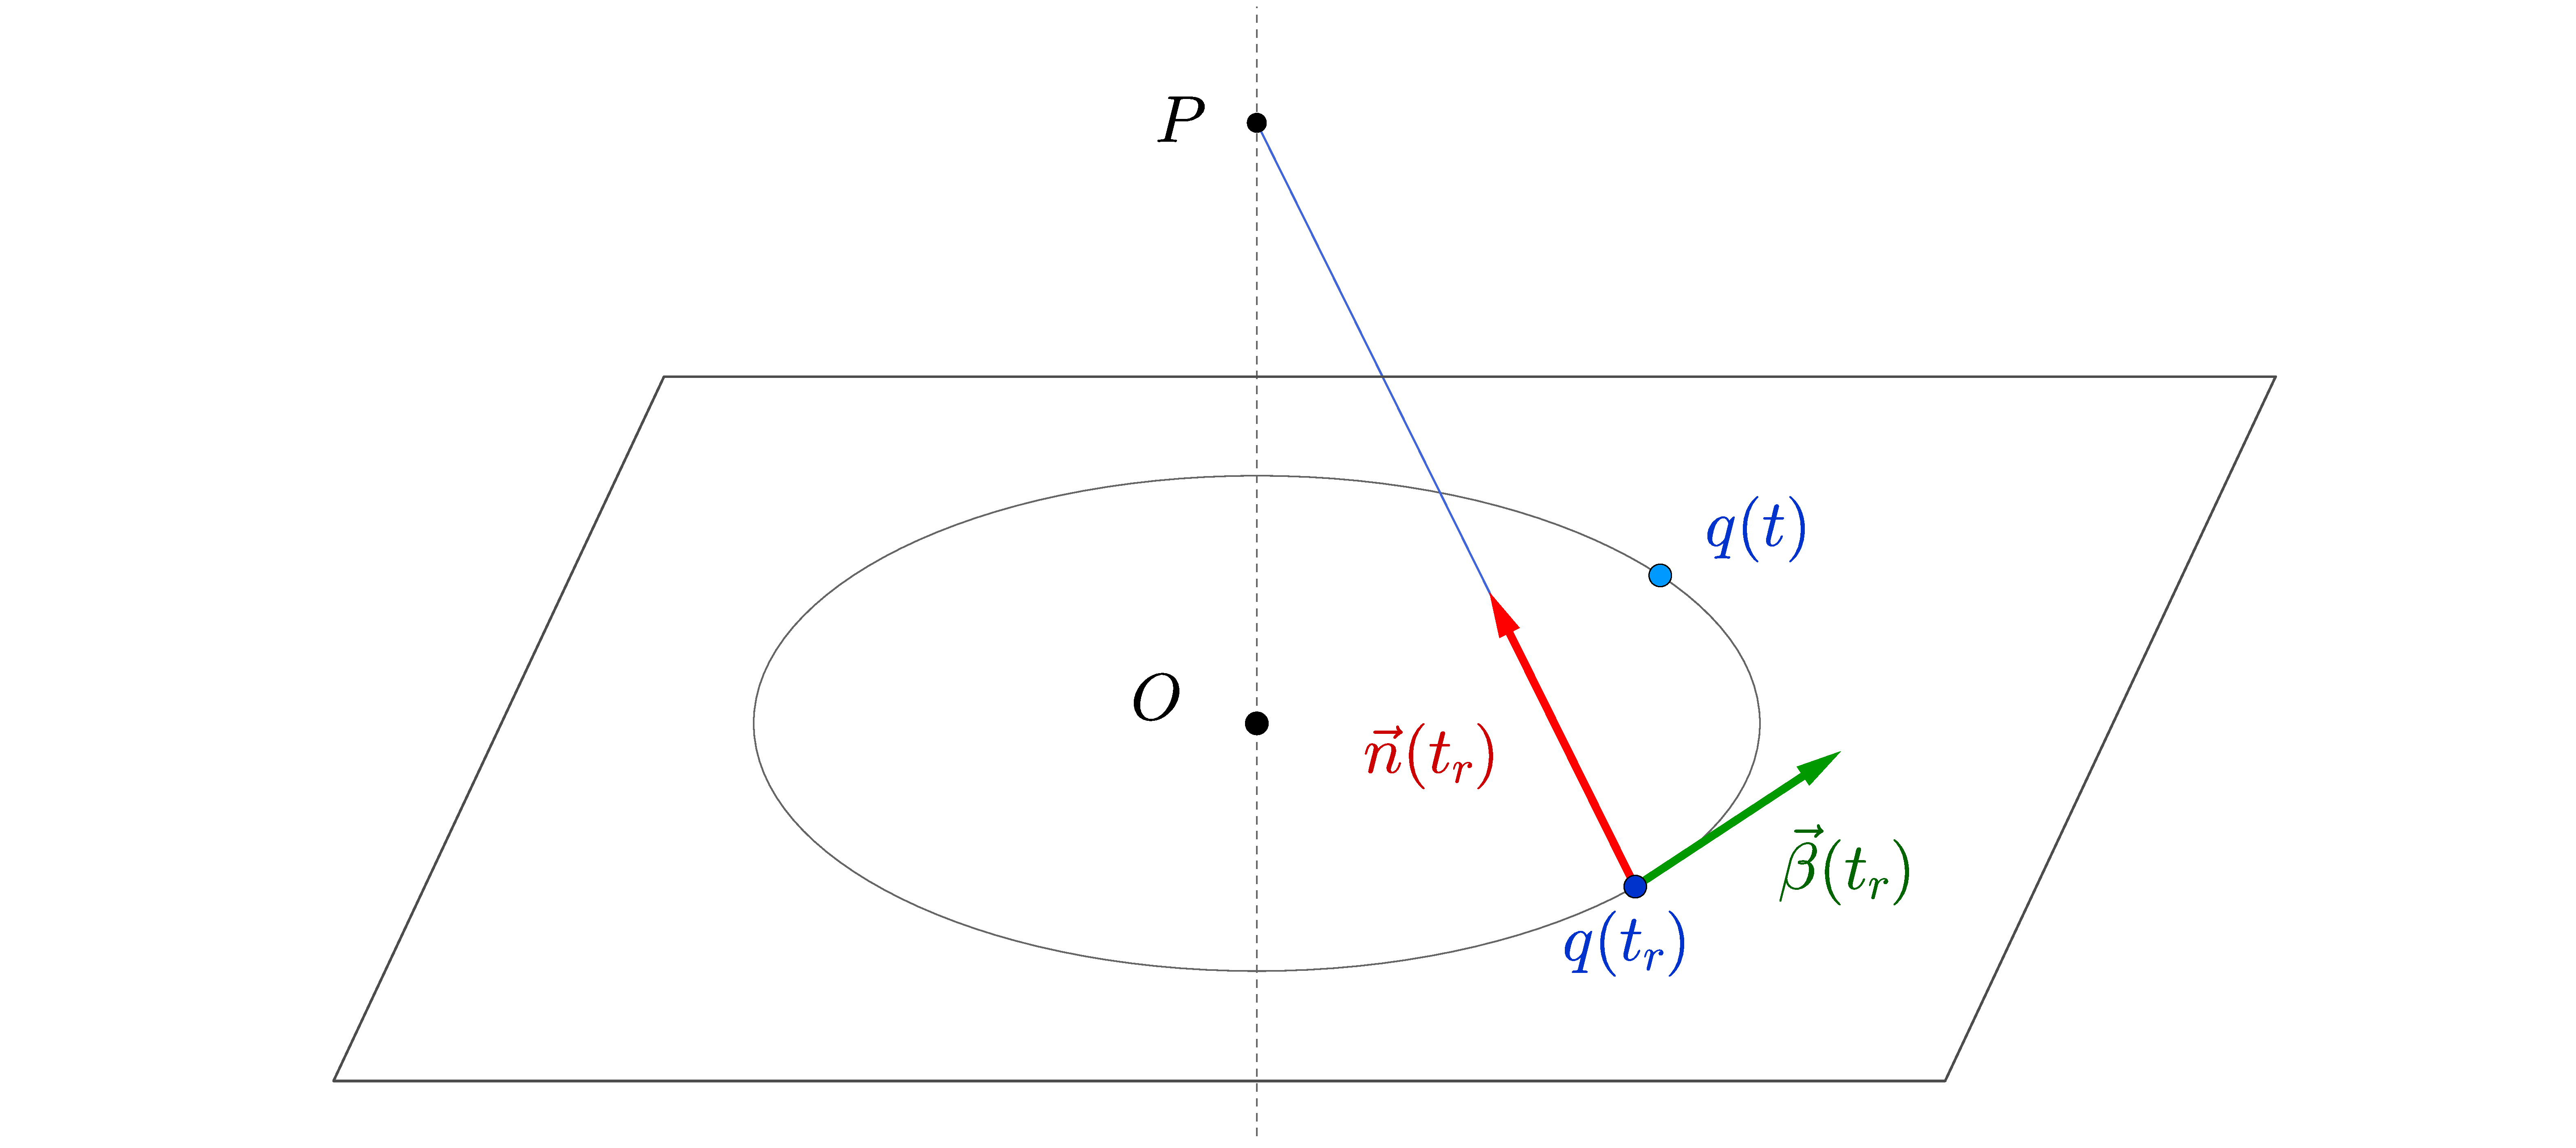
\includegraphics[width=\textwidth]{figura.eps}
    \caption{Representación gráfica del problema}
\end{figure}
Las expresiones generales de los potenciales de Liénard-Wiechert son:
\begin{subequations}\label{eq: Potenciales Lienard-Wiechert}
\begin{empheq}[left=\eqref{eq: Potenciales Lienard-Wiechert}\;\empheqlbrace]{align}
    \phi(\vec{r}, t) &= \dfrac{q}{4\pi \mathcal{R}(t_r)} \dfrac{1}{1 - (\vec{\beta}\cdot\vec{n})(t_r)}\label{subeq: Potencial escalar LW}\\ 
    \vec{A}(\vec{r},t) &= \vec{\beta}\phi(\vec{r}, t)\label{subeq: Potencial vector LW}
\end{empheq}
\end{subequations}
Como $\vec{r}$ se encuentra en el eje z y el movimiento de la partícula cargada es circular uniforme, se tiene: 
\begin{align}
    \vec{\beta}(t_r) &= \dfrac{\omega a}{c}\vec{u}_\theta (t_r)\label{eq:beta}\\
    \vec{n}(t_r) &\in \operatorname{Span}\{\vec{u}_r(t_r),\, \vec{u}_z\}\;\therefore\; (\vec{\beta}\cdot\vec{n})(t_r)= 0\label{eq: ortogonalidad beta y n} 
\end{align}
Donde $\vec{u}_\theta (t_r)$ se refiere al vector tangente a la coordenada polar para el tiempo retardado $t_r$. Por otro lado, como: 
\begin{equation}
    \mathcal{R}(t_r) = c(t-t_r) =\qty|\vec{r} - \vec{r}_q(t_r)| = \sqrt{z^2 + a^2}\label{eq: expresión de R}
\end{equation}
Esta relación se deduce fácilmente por la geométria del problema (Fig.). Cabe aclarar que  $r_q$ es el vector de posición de la partícula, y $\vec{r} = z \vec{u}_z$, que está dado por las condiciones del problema. Teniendo estas consideraciones en cuenta, la expresión del potencial vector \eqref{subeq: Potencial escalar LW} se reduce a: 
\begin{equation}
    \boxed{\phi(z,t) = \phi(z) = \dfrac{q}{4\pi \sqrt{z^2 + a^2}}}
\end{equation}
Donde, la independencia con el tiempo es consecuencia de la simetría cilíndrica y las posiciones sobre el eje de simetría elegidas. En cuento al potencial vector por \eqref{subeq: Potencial vector LW}: 
\begin{align}
\vec{A}(z,t) &= \vec{\vec{\beta}}(t_r)\phi(z) = \dfrac{\omega a }{c}\vec{u}_\theta(t_r)\phi(z)\label{eq: potencial vector, preliminar}
\end{align}
Por lo tanto queda determinar el tiempo retardado. Por \eqref{eq: expresión de R} se tiene: 
\begin{equation}
    t_r = t - \dfrac{\sqrt{z^2 + a^2}}{c}\label{eq: tiempo retardado}
\end{equation}
Por tanto, el potencial vector tiene esta forma final: 
\begin{align}
    &\boxed{\vec{A}(z,t) = \dfrac{q\omega a}{4\pi c\sqrt{z^2 + a^2}}\vec{u}_\theta \qty(t - \dfrac{\sqrt{z^2 + a^2}}{c})}\\ 
    &\boxed{\vec{A}(z,t) = \dfrac{q\omega a}{4\pi c\sqrt{z^2 + a^2}}\qty[\cos\qty(t - \dfrac{\sqrt{z^2 + a^2}}{c})\vec{u}_y - \sin\qty(t - \dfrac{\sqrt{z^2 + a^2}}{c})\vec{u}_x]}
\end{align}
\section*{Ejercicio 3}
Calcular los campos eléctrico y magnético en función del tiempo actual t, en el centro de la circunferencia del Ejercicio 2.
\Resolucion
La expresión general de los campos eléctricos y magnéticos de una partícula son: 
\begin{subequations}\label{eq: campos L-W}
    \begin{empheq}[left=\eqref{eq: campos L-W}\;\empheqlbrace]{align}
    \vec{E}(\vec{r}, t) &= \dfrac{q}{4\pi\gamma^2 (t_r)}\qty(\dfrac{\vec{n}-\vec{\beta}}{\mathcal{R}(1-\vec{\beta}\cdot\vec{n})^3})(t_r) + \dfrac{q}{4\pi c}\qty(\dfrac{\vec{n}\times\qty[\vec{n}-\vec{\beta}\times\dot{\vec{\beta}}]}{\mathcal{R}(1-\vec{\beta}\cdot\vec{n})^3}) (t_r)\label{subeq: campo electrico general}\\
    \vec{B}(\vec{r},t) &= \vec{n}(t_r)\times\vec{E}(\vec{r},t)\label{subeq: campo magnetico general}
    \end{empheq}
\end{subequations}
A las consideraciones \eqref{eq:beta} y \eqref{eq: ortogonalidad beta y n} se les añade las siguientes apreciaciones: 
\begin{align}
    \dot{\vec{\beta}} (t_r) &= -\dfrac{\omega^2a}{c}\vec{u}_r (t_r)\label{eq: betadot}\\
    \vec{n} &= -\vec{u}_r \;\because\; z = 0 \label{eq: n}\\
    \gamma^2(t_r) &= \gamma^2 = \dfrac{1}{1-\beta^2} = \dfrac{1}{1-\qty(\dfrac{\omega a}{c})^2}
\end{align}
Donde la expresión \eqref{eq: n} se debe al punto donde nos piden hallar los campos, i.e el centro de la circunferencia. Por tanto, podemos trabajar sobre el triple producto vectorial: 
\begin{equation}
    \vec{n}\times\qty[(\vec{n}-\vec{\beta})\times \dot{\vec{\beta}}] \overset{\eqref{eq: betadot},\eqref{eq: n}}{=} -\vec{n}\times\vec{\beta}\times\dot{\vec{\beta}} = \vec{u}_r\times\dfrac{\omega a}{c}\vec{u}_\theta\times\qty(-\dfrac{\omega^2a}{c})\vec{u_r} = -\dfrac{\omega^3 a^2}{c^2}\vec{u}_\theta 
\end{equation}
De esta forma el campo eléctrico \eqref{subeq: campo electrico general} tiene la siguiente forma: 
\begin{align}
    \vec{E}(\vec{0}, t) &= -\dfrac{q}{4\pi a^2}\qty(1-\qty(\dfrac{\omega a}{c})^2)\qty(\vec{u}_r + \vec{u}_\theta)(t_r)-\dfrac{q\omega^3a}{4\pi c^3}(t_r) = \nonumber\\
    &= -\dfrac{q}{4\pi a^2}\qty(1-\qty(\dfrac{\omega a}{c})^2)\vec{u}_r(t_r) - \dfrac{q}{4\pi}\qty(\dfrac{\omega}{ca}-\dfrac{\omega^3a}{c^3}+\dfrac{\omega^3 a}{c^3})\vec{u}_\theta (t_r)\nonumber\\ 
    &=-\dfrac{q}{4\pi a^2}\qty[\qty(1-\qty(\dfrac{\omega a}{c})^2)\vec{u}_r (t_r)+ \dfrac{\omega a}{c}\vec{u}_\theta (t_r)]
\end{align}
Además en el punto que se solicita, la expresión del tiempo retardado se reduce a $t_r = t- a/c$ de tal forma que la expresión final del campo eléctrico es: 

\begin{center}
    \framebox(0.9\textwidth,10em)[c]{\begin{minipage}{0.8\textwidth}
            \begin{align}
            \vec{E}(\vec{0}, t) &= -\dfrac{q}{4\pi a^2}\qty[\qty(1-\qty(\dfrac{\omega a}{c})^2)\vec{u}_r (t-a/c)+ \dfrac{\omega a}{c}\vec{u}_\theta (t-a/c)]  \\
            \vec{E}(\vec{0}, t)&= -\dfrac{q}{4\pi a^2}\left[\vec{u}_x\qty(1-\qty(\dfrac{\omega a}{c})^2)\cos(\omega t - \omega a/c) - \dfrac{\omega a}{c}\sin(\omega t - \omega a/c) + \nonumber\right.\\
            &\left.+\vec{u}_y\qty(1-\qty(\dfrac{\omega a}{c})^2)\sin(\omega t - \omega a/c) + \dfrac{\omega a}{c}\cos(\omega t - \omega a/c) + \right]
        \end{align}    
    \end{minipage}}
\end{center}

    
Aplicando la expresión \eqref{subeq: campo magnetico general} se tiene: 
\begin{align}
    \boxed{\vec{B}(\vec{0}, t) = \vec{n}(t_r)\times\vec{E}(\vec{0},t_r) = \dfrac{q\omega}{4\pi ac}\vec{u}_z} 
\end{align}
Donde de nuevo, la independencia en el tiempo es fruto de las simetrías y del punto estudiado. 
\end{document}